%% This document gives an example on how to use the ntnubachelorthesis
%% LaTeX document class.
%% Use oneside for PDF delivery and twoside for printing in a book style
%% use language english, norsk, nynorsk and one of the following shortenings
%%  ``BSP'' Bachelor i Spillprogrammering,\\
%%  ``BRD'' Bachelor i drift av nettverk og datasystemer,\\
%%  ``BIS'' Bachelor i Informasjonssikkerhet,\\
%%  ``BPU'' Bachelor i Programvareutvikling, \\
%%  ``BIND'' Bachelor i Ingeniorfad - data, \\
%%  ``BADR'' Bachelor i drift av datasystemer, \\
%%  ``BIT'' Bachelor i informatikk, \\
%%  ``BABED'' Bachelor i IT-støttet bedriftsutvikling.
%%   for example \documentclass[BIS,norsk,twoside]{ntnuthesis/ntnubachelorthesis}

\documentclass[BSP,english,oneside]{ntnuthesis/ntnubachelorthesis}

\usepackage{csvsimple}
\usepackage{booktabs}
\usepackage{minted}
\usepackage{pdfpages}
\usepackage{tabularx}
\usepackage{makecell}

\newcommand{\comment}[1]{\textcolor{blue}{\emph{#1}}}  %% use of the colour and you can see how to use commands with parts \comment{so what}

%% The class files defines these two
%% \newcommand{\NTNU}{Norwegian University for Science and Technology} %

% you can create you one #define like structures using the \newcommand feature
% you can change behaviour using \renewcommand

\newcommand{\com}[1]{{\color{red}#1}} % supervisor comment
%\renewcommand{\com}[1]{} %remove starting % to remove supervisor comments
% This will appear in text \com{Lecuters comment} and be visible unless you uncomment
% the renewcommand line.

\newcommand{\todo}[1]{{\color{green}#1}} % items to do
%\renewcommand{\todo}[1]{} %remove starting % to remove items to do

\newcommand{\n}[1]{{\color{blue}#1}} % other comment
%\renewcommand{\n}[1]{} %remove starting % to remove notes

\newcommand{\dn}[1]{} % add the d to a note to say that you have finished with it.


% Norwegian Characters,  needs the {} or to be separate from the next letters
% \o{}   \aa{}   \ae{}   so at the end of a word you can use \o  \aa   \ae
% \O{}   \AA{}   \AE{}   you can also just leave a space and latex will remove it
%    eg, NTNU i Gj\o vik  or NTNU i Gj\o{}vik

\begin{document}

\thesistitle{Conductor Hero - Process Report}
%\thesisshorttitle{} % use this if you have a very long title and want something shorter on the header pages
\thesisauthor{Rikhart Vigdal Bekkevold} %thesisauthorA, B, C etc
\thesisauthorA{Sabina Niewiadomska}
\thesisauthorB{Per-Morten Straume}
\thesisauthorC{Ida Ellinor Syverinsen}
\thesisauthorD{Andreas Wang}
\thesisauthorE{Yijie Zhou}

\nmtkeywords{Process Report, Reflection, Teamwork}
% TODO: Write Abstract!
\nmtdesc{
Experts in Teamwork is a course where students from various disciplines are put together in a team to work on a project throughout the semester. For the course, our group worked on a VR game called Conductor Hero where the player takes the role of a Conductor in a fantasy environment. This document gives and overview over our experiences, thoughts, sitatuations, and feelings.
}


\nmtoppdragsgiver{\NTNU}
\nmtcontact{Andreas Wang, andrwan@stud.ntnu.no, 48048162}

\thesisdate{\ntnubachelorthesisdate}
\useyear{04.05.2018}

\nmtappnumber{0} %number of appendixes
\nmtpagecount{} %currently auto calculated but might be wrong % this is the file which contains all the details about your thesis

\makefrontpages % make the frontpages

\tableofcontents
\listoffigures
\listoftables
%\listoflistings

\chapter{Introduction}
The course Experts in Teamwork (EiT) is designed to give students experience with cross disciplinary projects to enhance their communication and collaborative abilities, preparing them for the challenges they will meet in their future work environments~\cite{ntnu_what_is_eit}. 

We took part in the village “Virtual and Augmented Reality for Games, Health and Education” which focuses on the exciting new possibilities of virtual and augmented reality. As this is a young field we were given the opportunity to experiment with different ideas, with the potential of shaping the future of virtual reality (VR) and augmented reality (AR). 

Our project, Conductor Hero, is a VR rhythm game that introduces the player to the world of ensemble conducting. The project was an exciting first hand-experience of the challenges faced in virtual reality, and also presented us with the requirements of working in a cross disciplinary team. This document will give the reader an overview over the situations, reflections and experiences we encountered throughout the semester.


\section{Group formation}
\subsection{Animal Model}
The 6-animal model, developed by Simon McCallum~\cite{six_animal_model}, focus on the different roles of group members. The model uses six animal avatars (bear, wolf, cat, puppy, owl, and rabbit) to represent the different roles, creating a cognitive distance between the role and the individual, helping with group organisation and communication. The bear is the group leader, while the wolf is the manager ensuring that everyone in the group is participating. The cat takes on the role of the critic, looking for flaws in proposed ideas, with the puppy being the complete opposite, enthusiastic and supporting of every idea. The owl has the role of the processor and ensures that objectives are met, and finally the rabbit acts as a facilitator, volunteering to get coffee or other resources needed by the group. In this model every animal is considered equally important for group success.

During the first village day the each student was encouraged to identify themselves with one of the 6 animals. The people who identified as bears were told to stand up, and the others were told to form groups with the different bears. These groups should ideally have a good mix of the different animals. Through this exercise we ended up with our group, consisting of
Per-Morten (bear), Andreas (owl), Yijie (puppy), Rikhart (cat), Sabina (rabbit), and Ellinor (wolf). 


\subsection{Assigning roles} \label{sec:assigning_roles}
After forming groups based on the 6-animals model, we performed a triangle exercise. An image from the exercise can be seen in Figure~\ref{fig:triangle_exercise}. Here, each group member were given the chance to inform the others what they could bring to the project, in terms of personality,  practical experiences and theoretical knowledge. An overview of the skills can be seen in Table~\ref{table:skills}

\begin{figure}[h]
    \centering
    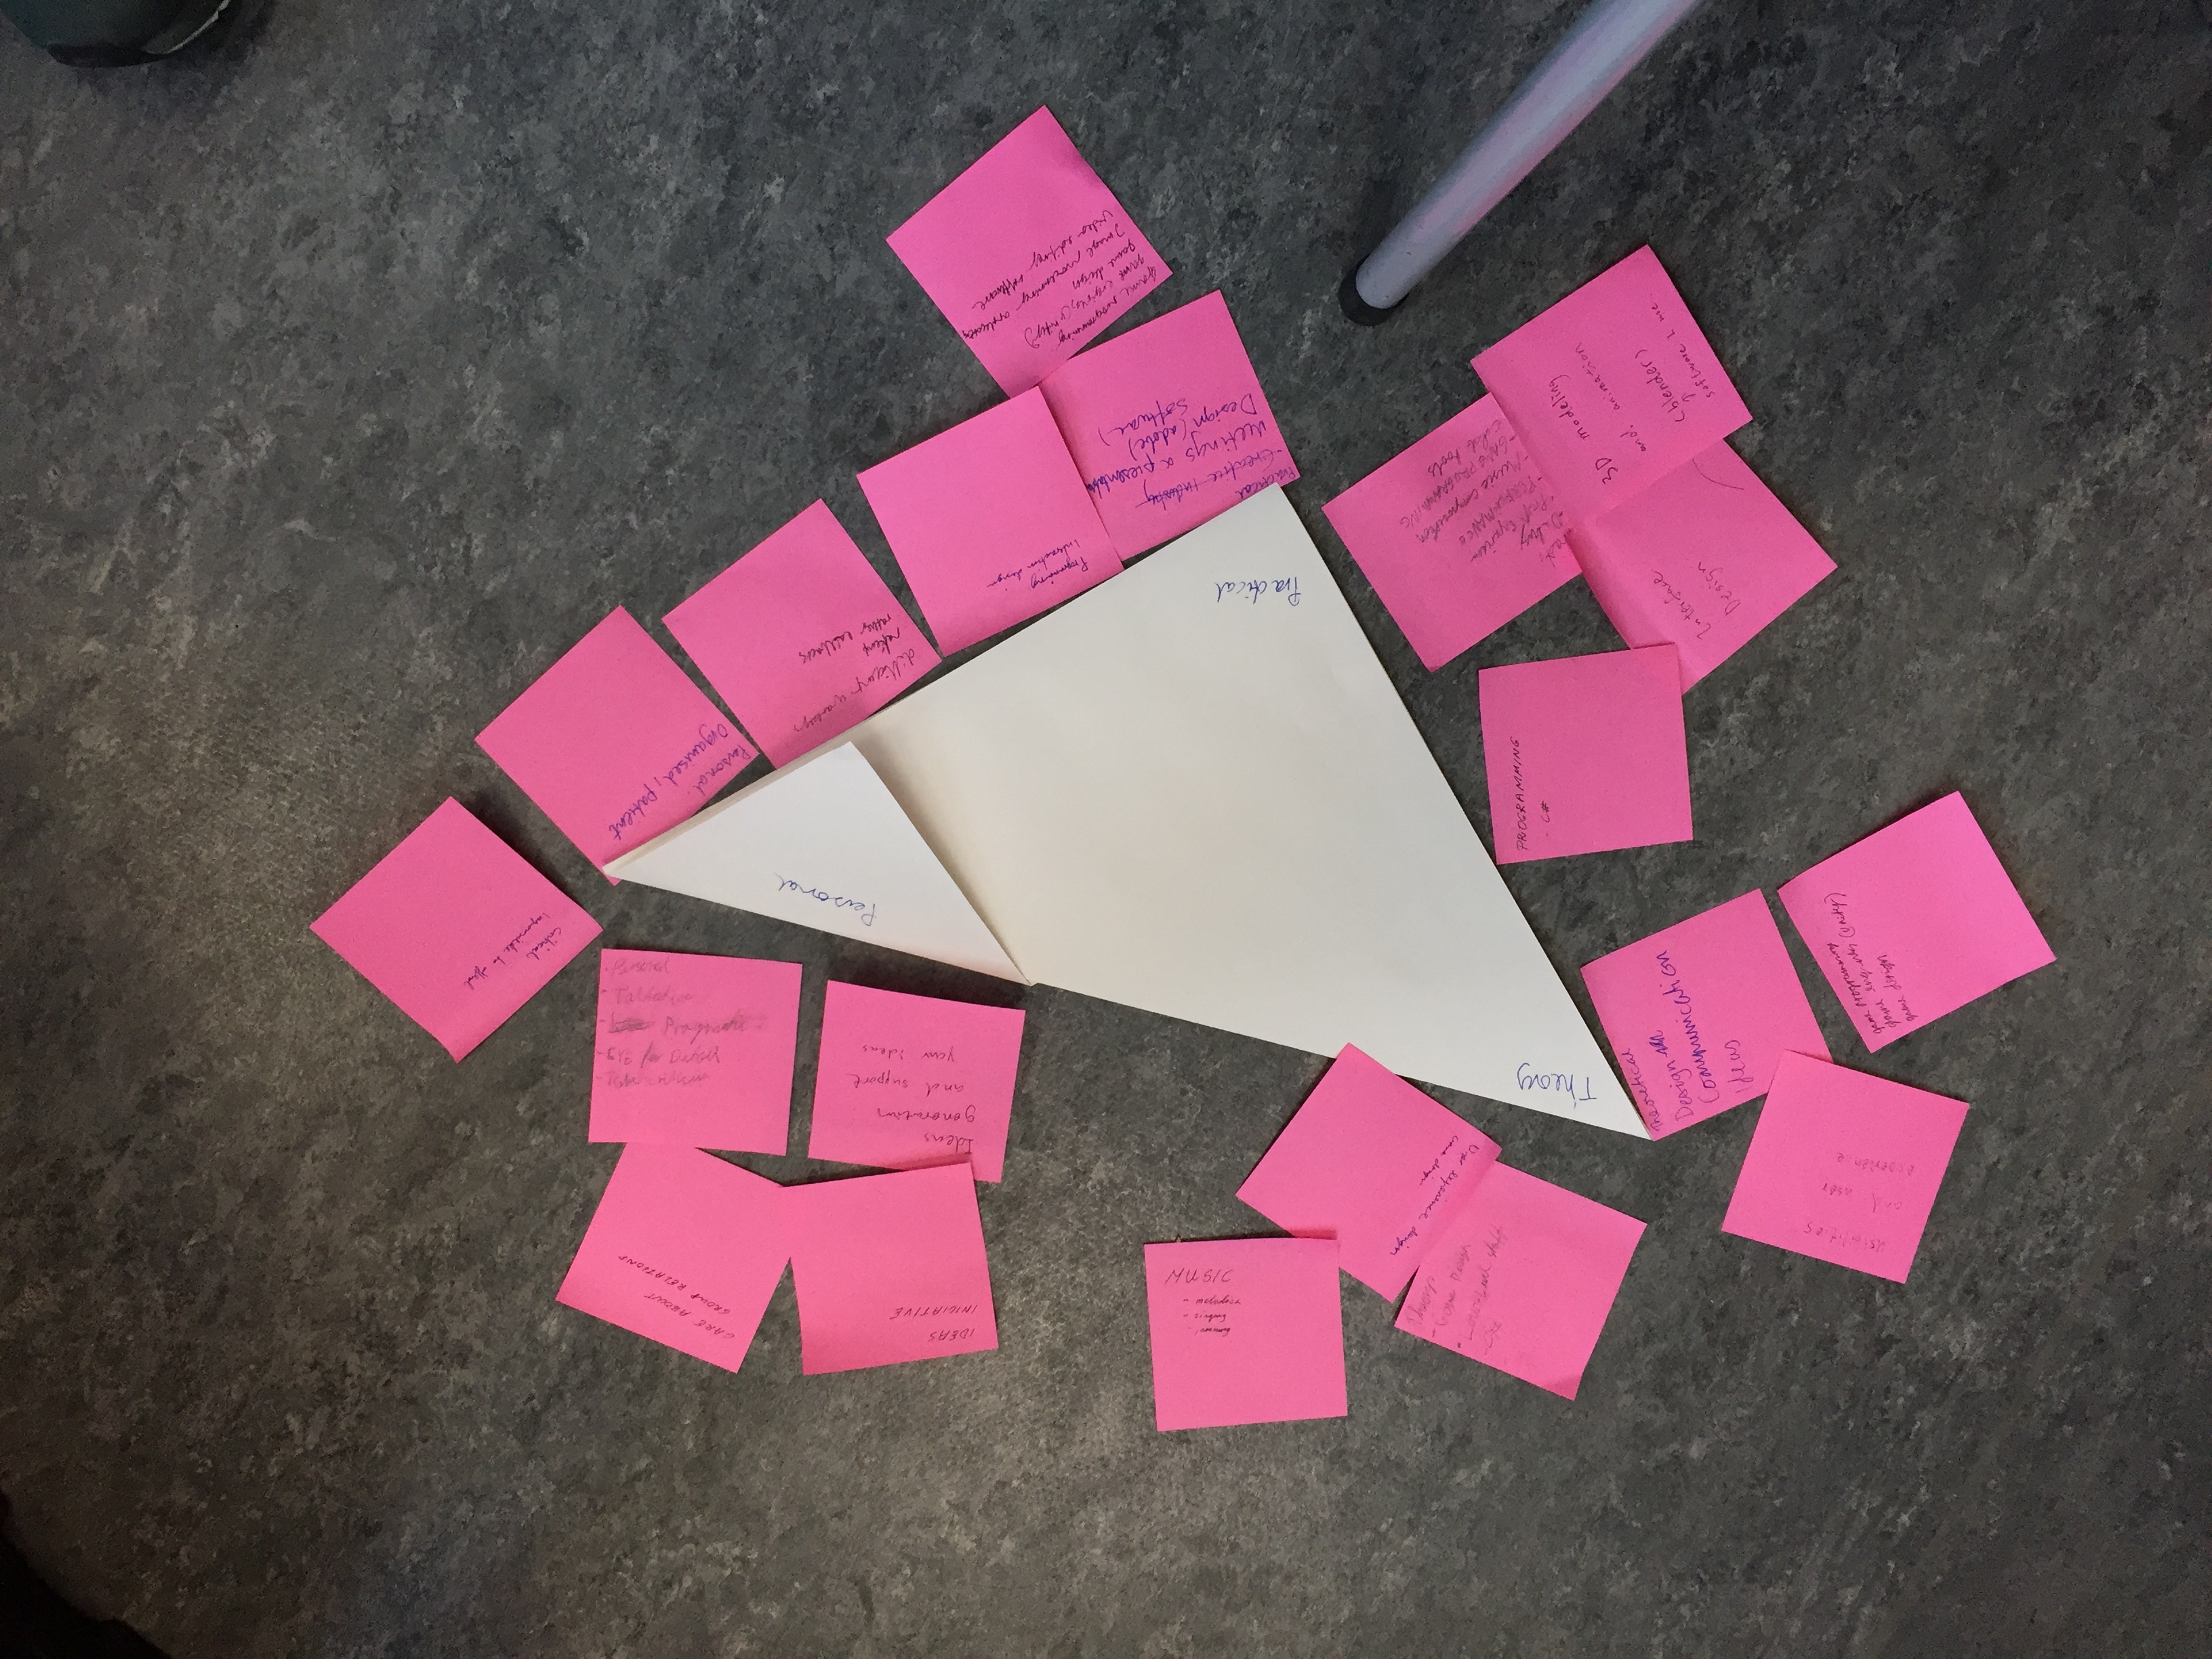
\includegraphics[width=0.9\textwidth]{images/triangle_exercise}
    \caption[Exercise for surveying skills within the group.]{Exercise for surveying skills within the group. Each triangle corner: the type of value. Post its: the values team members contribute to the group. The exercise depicted formed the basis for the table below.}
    \label{fig:triangle_exercise}
\end{figure}

\begin{table}[H]
    \centering
    \begin{tabularx}{\linewidth}{ | l | X | X |}
        \hline
        \textbf{Member} & \textbf{Skill} & \textbf{Background}  \\
        \hline
        Rikhart & Design, Programming, Critical thinking & Web Development, Interaction Design \\
        \hline
        Sabina & Design, Programming, Music & Web application development, Interaction Design \\
        \hline
        Per-Morten & Programming, Music Composing & Game Programming, International Marketing \\ 
        \hline
        Andreas & Programming, Experience with the Unity Engine, Music & Game Programming  \\
        \hline
        Yijie & Design, 3D modelling, animation & Digital Media, Interaction Design \\
        \hline
        Ellinor & Design, Graphics design, Music & Graphic Design, Art direction, Interaction Design  \\
        \hline
    \end{tabularx}
    \caption{Table of the groups skillset.}
    \label{table:skills}
\end{table}

After performing the exercise, we had a better awareness of each others personalities and skills, and established more specific roles for our group. Ellinor took the role of project lead, as she was interested in exploring her leadership potential, and Per-Morten was happy to pass on the role. Yijie, had experience with 3D modeling and animation and therefore took the role of art director. Per-Morten, who had a strong leadership skill and an interest in software architecture took the role of technical lead. Andreas took the role of Unity expert as he had the most experience with the Unity game engine. He was also given the responsibility of taking notes to record the process and progress of the group. As Sabina and Rikhart had backgrounds in both development and design it was decided that they should work as bridges between the designers and programmers. Additionally, Rikhart was delegated the role of UI expert, based on his previous experience within the field. Sabina volunteered to take the role of public relationship manager, as we intended to contact several external professionals.
% TODO: UPDATE after changes are done
\section{Group Members}
\begin{figure}[tpbh]
    \centering
    \includegraphics[width=0.9\textwidth]{images/Conductor_team}
    \caption[Group Photo]{Our group, 24 eyes}
    \label{fig:conductor_team}
\end{figure}
Below follows a more in-depth overview of the group members (shown in Figure~\ref{fig:conductor_team}), and our thoughts going into the project.
\subsection{Rikhart Vigdal Bekkevold}
\textbf{Nationality:} Norwegian \\
\textbf{Study:} Master in Interaction Design \\
\textbf{Background:} Web Development, Interaction Design \\
\textbf{Role:} Cross-discipline communication, UI expert

Entering this project I already knew that I was a very critical person. I have always seen this as a benefit when it comes to seeing the holes in ideas and in identifying problems. I have also experienced that it can be a less positive thing if it is dominating, hindering progress and creating conflicts in groups I have partaken in. Knowing this in advance, it was something I tried to work on, and to make sure it didn’t become too dominating in our groupwork. Before this course I had been in many different groups, ranging in success from bad to decent, but never good. Because of this, group work had always been a chore to me.


\subsection{Sabina Niewiadomska}
\textbf{Nationality:} Polish \\
\textbf{Study:} Master in Applied Computer Science \\
\textbf{Background:} Web application development, Interaction Design \\
\textbf{Role:} Cross-discipline communication, Public relations

I joined the EiT course with both experiences from students projects and work. In students projects, it often happened that I become a leader, students with which I was cooperating were describing me as "person bringing initiative" or "good coordinator". In the real work environment, I've never had a  chance to become a team leader.In the first classes, we were asked to represent ourselves as a type of animal. Knowing my duties this semester I decided that I would like to take a role of a wolf or an owl. Some people were suggesting that I would be a good wolf (good work coordinator) and some that I would be a good owl (I like to organize group work with tools like Microsoft Planner/Trello/SharePoint ). Unfortunately, when I joined this group the positions of wolf or owl were already taken, but it wasn't a problem for me. As a result, I was assigned the rabbit role. Before EiT course I was totally unfamiliar with Virtual and Augmented Reality products and development process. I don't play any games regularly. My programming skills are strong in rapid software development in ASP.NET for financial applications (both desktop and web solutions, but mostly web development). I also have a good understanding of databases problems and a strong interest in User Experience issues. One of the biggest challenges of this project was to learn the concept of game programming and Unity for Virtual and Augmented Reality.

\subsection{Per-Morten Straume}
\textbf{Nationality:} Norwegian \\
\textbf{Study:} Master in Applied Computer Science \\ 
\textbf{Background:} Game Programming, International Marketing \\
\textbf{Role:} Chief Technical Officer

Before taking the course I already had a fair amount of group experience, both mono-discipline and cross-discipline projects, in professional and academic settings. Because of this I already had some ideas of my behavior in groups, and how it affected group dynamics. I was aware that I can be dominating in group, and also that I can be quite vocal and honest about my views. However, I always try to be open to others views, and promoting discussions to reach optimal solutions to problems. My wish for the course was that if I was completely wrong about my theories of myself in group dynamics I would be made aware of them.

Throughout my higher education I usually ended up being the leader in group projects, mainly because no one else wanted to. However, I have never been really comfortable with this role, and decided for this project that I did not want to be project lead. One of the reasons for this is that I often struggle with several managerial tasks like structuring and planning because of my ADHD diagnosis. Nonetheless, I did volunteer to be a bear on the first village day, as there were not that many students who seemed interested in the role.


\subsection{Ida Ellinor Syverinsen}
\textbf{Nationality:} Norwegian \\
\textbf{Study:} Master in Interaction Design \\
\textbf{Background:} Graphics Design, Art Direction, Interaction Design \\
\textbf{Role:} Chief Executive Officer

At the beginning of the course I decided to keep an open mind to the project, even though I had heard mixed, and often negative, opinions about the course from other students. During the group formation, I picked “wolf” as my primary animal character, with “cat” as a second option. I found this fitting as I am not afraid of voicing my opinion, and can sometimes enjoy playing “Devil’s advocate”. I decided to try to join a group where I had not previously worked with any of the other group members, which I managed to. 

I already had a lot of experience working in groups before starting this project, both from educational and professional settings. This also includes the first half of my master programme, in which all courses have included group projects. My experiences with group projects have mostly been positive since commencing higher education, and I consider myself to be well versed in teamwork. I am, however, also aware that I am a typical “introvert”, meaning that working with, and also spending time with, others can sometimes make me feel more tired and “drained” than working individually. 


\subsection{Andreas Wang}
\textbf{Nationality:} Norwegian \\
\textbf{Study:} Master in Applied Computer Science \\
\textbf{Background:} Game Programming \\ 
\textbf{Role:} Unity Engine Expert

Prior to entering the project I already had a fair amount of experience working in various groups. Some of these were relatively well performing while some also were dysfunctional. I already knew the importance of teamwork for larger projects due it being central for game programmers. It was exciting to hear that we were going to work on VR/AR applications in this course and I was interested in seeing how cooperating across disciplines would work as this is something that has not been a part of my previous education. 

\subsection{Yijie Zhou}
\textbf{Nationality:} Chinese \\
\textbf{Study:} Master in Interaction Design \\
\textbf{Background:} Digital Media, Interaction Design \\
\textbf{Role:} Art Director

Before the EIT course, I have gotten used to working in multidisciplinary teams both for school projects and in the real working environment, though I never pay attention to the team, theories about teamwork, or my role in the team. During my previous projects and working experience, I used to think that maintaining the team was not my responsibility and just focused on my own work. For conflicts I encountered, I usually just let them go and didn’t try to handle them properly. Generally, I cared more about my personal work than the group work. This made me less active during the group discussion and I sometimes lost the big picture of the group work. I was aware that though I was always willing to contribute to the group and try my best to accomplish my tasks, ignoring the group is definitely harmful both for myself and the group. I hope that during this course, I could improve the defects mentioned above and focus more on the group. Additionally, I hope to be able to have more opinion exchanges with other group members and contribute ideas more actively. 
 
\chapter{Creating a Successful Group}
While Experts in Teamwork frequently focuses on dealing with the challenges of working in cross-disciplinary groups, we also looked at some prerequisites for creating successful groups in the first place. Some of the measures we took internally to ensure a well-functioning group are described below. 
\section{Group Goal}
According to Johnson et al.~\cite{2013johnson} effective groups state clear goals and strategies to achieve those goals. At the start of the project, our team agreed on a common goal - achieving the best possible grade. We also aimed to create a substantial prototype which could potentially be added to our own portfolios. During first meetings we spent a lot of time trying to reach a common understanding of the game we were developing and how we could achieve our goals. We divided tasks among team members close to their interest which let us be committed to the group goal. 
\section{Group Rules}
Another characteristics of effective groups which is mentioned by Johnson et al.~\cite{2013johnson} is effective communication to reduce misunderstandings. 
Our group contract dictated that we should use Discord\footnote{\url{https://discordapp.com/}} for communication, which we were required to check daily. We also defined teamwork climate rules, like how criticism should always be constructive. 
We also stated that if someone had a problem regarding our project this person should inform members as soon as possible and as that we should try to help as a group. 

Equal participation, shared leadership and members’ power based on expertise, ability and access to information is the next characteristic mentioned by Johnson et al.~\cite{2013johnson}.
In our group contract we agreed on the decision process and group members roles.
We decided that large, impactful decisions should be made by all group members, while smaller decisions would be made by the technical leader and art director.

\chapter{Results} \label{chap:results}
In the duration of the course we created a prototype for the game Conductor Hero (see Figure~\ref{fig:conductor_hero}). A fully playable prototype for a VR conducting game. The game is available at GitHub\footnote{\url{https://github.com/Per-Morten/imt4310_conductor_hero}} and a video demonstrating the gameplay can be found on youtube\footnote{\url{https://www.youtube.com/watch?v=YQQTDyfQb-Q}}. 
We discovered through the creation of this game that the group worked well together, and low number of conflicts and a high amount of cooperation.
\\ 
\begin{figure}[tpbh]
    \centering
    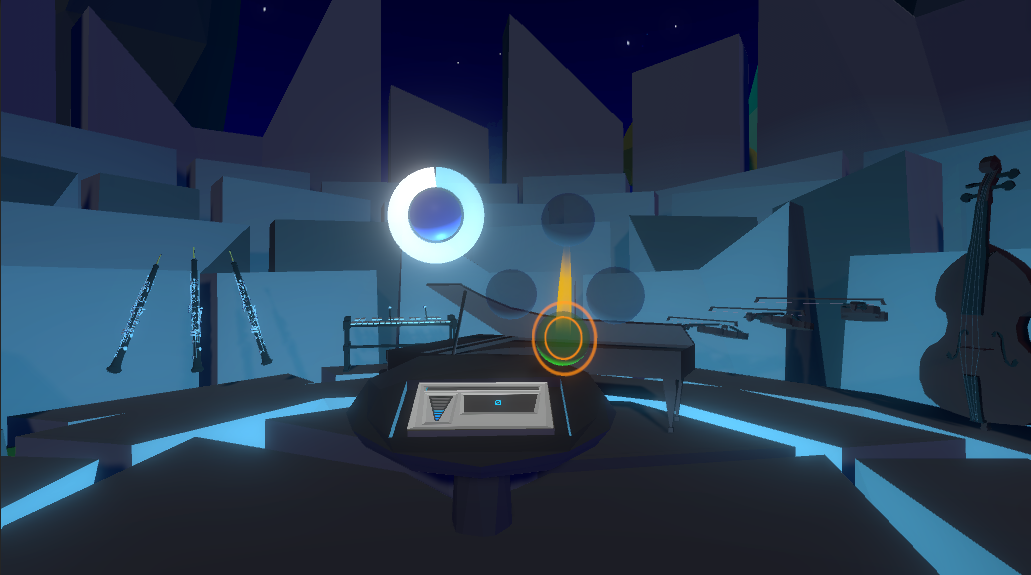
\includegraphics[width=1.0\textwidth]{images/cue}
    \caption[Conductor Hero]{A screenshot of the final Conductor Hero prototype}
    \label{fig:conductor_hero}
\end{figure}
\chapter{Discussion} \label{chap:discussion}

\chapter{Reflection}
An important part of the course has been the development of our ability to reflect on our own and others behaviour when working in groups. Reflection, both individually and as a group, can serve as a tool for personal and group development. 

Personal and group reflections were written each village day. A brief summary of group and personal reflections are provided below.

\section{Group Reflections}
Exercises were introduced early in the course, at a time where the group members were not familiar with each other. Because of this they felt forced and artificial, giving us a bad impression that stayed with us throughout the project. A common theme throughout the group reflections was that the course exercises did not give us any major insights. In retrospect we should probably have been more open to the exercises, as we got the feeling that some of the other groups found them beneficial. 

During the exercises, we still found the results to be descriptive of the dynamics in the group. While this was interesting, and helped us identify problematic patterns, we also felt like the exercises reinforced our already existing traits, rather than solving any problems. 

We acknowledged several times throughout the project that we all felt safe within our group, both in terms of presenting ideas, and vulnerabilities. However, there was an imbalance in who was talking the most in the group. While we believe that such an imbalance can be unhealthy, in our case we consider this to be the natural result of the group members’ personalities. As long as everyone’s opinion is considered, and the more quiet group members are allowed to talk, we consider this unproblematic. Additionally, we felt safe in relation to finishing tasks on time, allowing us to delegate work and rely on each group member pulling their weight.

Throughout the project we managed to achieve a lot of the goals we had set for ourselves, indicating a good workflow. The daily meetings kept every group member updated on individual and group progress, and reduced the need for disrupting others’ work later in the day leading to unnecessary discussions. At the same time these discussions were welcome if needed.

\section{Individual Reflections}
\subsection{Rikhart Vigdal Bekkevold}
The group consisted of both programmers and designers. I had a background in web development, comprising of both design and programming, so I had experience in both fields. As a consequence of this, I did not have the same learning outcome in terms of developing my cross-disciplinary skills and understanding, as the others might have had. I already could communicate well with both fields so I didn’t experience any conflicts that could arise from this.

A “1+2” exercise, midway through the course, forced us to give feedback about each other (1 negative and 2 positive). During this exercise the other members told me that I could present my views, and argue, very strongly (arguing strongly, not as a general behaviour), something that was described as “off-putting” at times. I was already aware of this tendency, but I never knew how people viewed it or felt about it. The strength of this task was that it forced us to share thoughts about each other, something we often try to avoid, and I learned something about myself I might not have otherwise.

Unfortunately this was all the usefulness I got out of the exercises we did, the group functioned too well to benefit from these exercises which mainly seemed aimed at non-functioning groups.We had too few, and mild, conflicts for me to learn much from them. In the end I felt that I didn’t really learn anything new about myself that I didn’t already know, so very few comments from the others (in relation to me), surprised me.

A beneficial part of this course for me was observing the behaviour of the other group members, and how their behaviour affected the group. I learned a lot from seeing how the other members dealt with situations and how they acted in relation to each other and to me. I observed that: They blamed themselves first, they didn’t overestimate their abilites, they respected others opinions, they worked hard, they saw others perspective, they explained their motives and reasoning, delivered their criticism in a considerate way and were helpful and friendly. Although I believe I can credit myself with some of these qualities as well, by seeing the great qualities of the others, it taught me that I still have lots of room for improvement when it comes to being a good group member.
 
In the future I will take the aspects/qualities of this group that made it work so well and apply in future groups. Hopefully I can use this to make the bad, conflict filled, group experiences of the past; better in the future. I will also remember that people don’t always tell you what they think and be wary of my sometimes overly strong arguing. 

\subsection{Sabina Niewiadomska}
During the course, I had a chance to get to know game programming, as well as how the graphics part is connected to the programming part. I was surprised that so many elements of a game are not programmed but just build into Unity. I think that the theory provided by the course on how to create a well-functioning team is interesting but I believe the course will not help much into a real work related situations, no one of exercises seemed to be applicable in a workspace and the course also didn't teach us how to soften critical situations. 

The course didn't fulfill my curiosity about successful group communication, therefore I will continue my personal research on that topic. After the course, I'm more open for game programming, but still, I'm not encouraged to play any games. 

However, the course was enjoyable experience in terms of project creation.

\subsection{Per-Morten Straume}
Throughout the exercises and feedback given I was happy to discover that most of my perceptions of myself in groups was largely correct.
I was also happy to notice that I didn’t really have any difficulties communicating with the group when it came to cross-disciplinary issues. I often understood what other group members was talking about, and in the cases where I didn’t I had no problem asking for clarification. This also seemed to be the case with the other group members, ensuring that most of the time we were all on the same page, which is vital for group projects like these.

The unpredictable structure of the village days and our erratic group meetings became a frustration to me, as I need a predictable and structured work environment to stay focused and productive. Luckily the team was understanding and accepting towards this challenge leading to a satisfactory solution with chunked work times. 

While the course didn’t leave me with any newfound revelations of how I function in groups, it did strengthen all my existing theories, which I will bring with me.
In the future I will be even more aware of my often dominating role in groups, and the positive and negative effects that role brings. I will be more vary of the consequences of my desire to be direct, honest, and “to the point”, and how it might affect the group dynamic or influence the groups opinion. I also found that while I don’t like being the overall leader of a project, I don’t have any problem acting as a more specialized leading role, like technical director. Additionally, I have gained valuable experience in how I can play to the strengths of my diagnosis, but also the importance of predictable schedules, and getting help to structure and plan any non-product related activities. Because of this experience I will be more open about my diagnosis in future team projects to achieve greater productivity.

\subsection{Ida Ellinor Syverinsen}
After the initial group formation and exercises, I was selected to be the leader of the group. I considered this to be a great vote of confidence, and I found filling this role to be a new and very interesting experience. As I do know that I sometimes can be a little too focused on details, I used this as an opportunity to practice not micro-managing design (or other) decisions, but to instead delegate tasks and responsibilities. 

It is possible that a lack of conflicts in the group have limited my learning, but it has been hard to find “difficult situations” to reflect about as, in my opinion, all group members involved themselves in the process, stayed positive, and contributed their share (and more!) to the project. Not surprisingly, the group had a few discussions where communication across disciplines created a few minor misunderstandings, but these were resolved quickly and I would not describe any situations within the group as “conflicts”. Overall, I found the group work very rewarding, and it was exciting to create a project for VR technology. 

The theory and exercises presented in the course curriculum have no doubt been interesting, but to me they seemed to be more useful for groups with high levels of conflict. I have personally found the discussions with the course coordinator and student assistants to be both more interesting and more valuable for my own learning. 

While I do not believe that the way I behave in groups have changed significantly during this course, I think that I have become somewhat more aware of the needs and behaviours of other group members, as well as the dynamic between other group members. I believe that Expert in Teamwork have increased my interest in leadership, and that I am now more likely to pursue positions of leadership in the future. 

\subsection{Andreas Wang}
While working on the project I learned a fair amount of various things. I got experience in working with a fairly diverse team which is closer to what you would find in a real world company. As part of this, I acquired more experience in integration of components from the various disciplines to make sure everything worked together in the final product. 

As part of working in a team with high diversity I also learned the importance of making sure that everyone is on the same page during discussions as members from different disciplines might use the same or similar terminology, but with different meanings. 

The course taught us a good amount of theory around how to structure and deal with situations in dysfunctional teams which is useful knowledge to have in the future, but the focus feels to be a bit too heavy on this end and and it almost feels like it is expected that most groups will have their fair share of conflicts and issues. If a group already is dysfunctional in the real world I am also unsure if everyone in it would want to do the presented exercises in the course. While the theory was nice, I would have liked to see some more concrete examples of how to deal with group dysfunctionality as well. At the same time, doing this course has made me think more about previous group experiences(even teams/groups in games!) and reflect better on what went well or badly which I find pretty valuable. 

A problem I had with a fair amount of the group exercises was that they were placed too early in the course at a point where the group had done very little actual work and the members did not know each other very well. Due to this it was not easy to give meaningful feedback to each other. This was particularly apparent with exercises like 2+1 as it was hard to provide positive and negative feedback when you barely know each other. It would probably beneficial to put these early exercises a bit later on in the course so there is more for the group to discuss. 

In general, this is the most well functioning team I have worked with of this size in any course so far. While having such a well functioning team seems a little bit out of place in relation to what the course seems to expect, I feel like we still learned a lot from reflecting on why everything went as well as it did. On a more technical end I ended up getting experience with using the SteamVR library in combination with the HTC Vive which definitely can be useful for the future as VR becomes more mainstream. 

I do not feel like I really learned anything new about myself and how I interact in groups as I already self reflect a fair amount. I already knew that I do not speak a lot, especially early on in new groups as I do not know everyone just yet, but also that I will speak my opinion on something if I deem it necessary. 

I feel like the major takeaway from this course for me is partly the experience of working in a diverse team which is more representative of teams you will find in the real world. The things we have learned in the course can also be useful in the future to reflect more around the actual team itself and not only its individuals. I do not think that there is a “one size fits all” solution for every group out there, but there are valuable components of the various pieces of theory from the course which could be applied to other groups in the future.

\subsection{Yijie Zhou}
Throughout the course, two most significant learning outcomes for me are how to handle group diversity and the use of group rules. We learnt and practiced various theories and methods around group diversity in this course, including form a heterogeneous group, benefits and damages of diversity, manage potential conflicts caused by diversity, etc. As a designer in the creative industry, it is naturally required to work in multidisciplinary teams, where diversity commonly exists. Therefore, I think being able to deal with the group diversity in a proper way and take the advantages of a diversified team can be a useful skill in the future. These outcomes are also helpful when you are in a leadership position, giving you the insight to recruit teams with a decent amount of diversity which is suitable for your project. 

The second useful skill for me is to introduce the group contract and group rules in the teamwork. With the group contract, members can have better awareness about the common goal and work in the same direction. Since group rules are established based on group members’ agreement, when conflicts happen, it can provide a solution which is acceptable for every group member. This can focus the group on the task and avoid personal conflicts, which has a relatively higher harmful influence on the teamwork. For example, if one member comes out with an idea which does not correspond to the common goal, instead of saying it is a bad idea, which may cause unnecessary argument in the team, others can reject the idea based on the group contract. I think using group rules are helpful both in school projects and the real working environment.

In addition, this course also provided an opportunity to improve my expertise. I explored 3D interaction in the VR environment and sharpen my 3D modelling skills. While working with experienced game developers, I grasped the fundamental concept of game design and had a better understanding of the collaboration between Blender and Unity. Since our project is an ensemble conducting game, I also gained more experience in the orchestral music and had a better understanding of conducting.

I will keep the useful skills from the course with me in the future teamwork. With a more holistic view of the team and various theories of teamwork, I would like to try to take more responsibilities in the group and challenge myself for positions which require a higher level of leadership. Also, I feel personal reflection is a good way to have a better understanding of myself and my position inside the group, and I will keep this as a habit. 
 
\chapter{Conclusion}


\bibliographystyle{ntnuthesis/ntnubachelorthesis}
\bibliography{inc/ref}

\appendix %after this line all chapters will have letters instead of numbers
% spreadsheet data?

\end{document}
